\section{Analysis package validation}
\label{sec:validation}

\subsection{Candidate selection and invariant distributions}
\label{subsec:invMassValidation}

- Ds/Lc in pp MC: invariant mass from task, invariant mass from bit, invariant mass from pandas applying standard cuts

\begin{figure}[tb]
\begin{center}
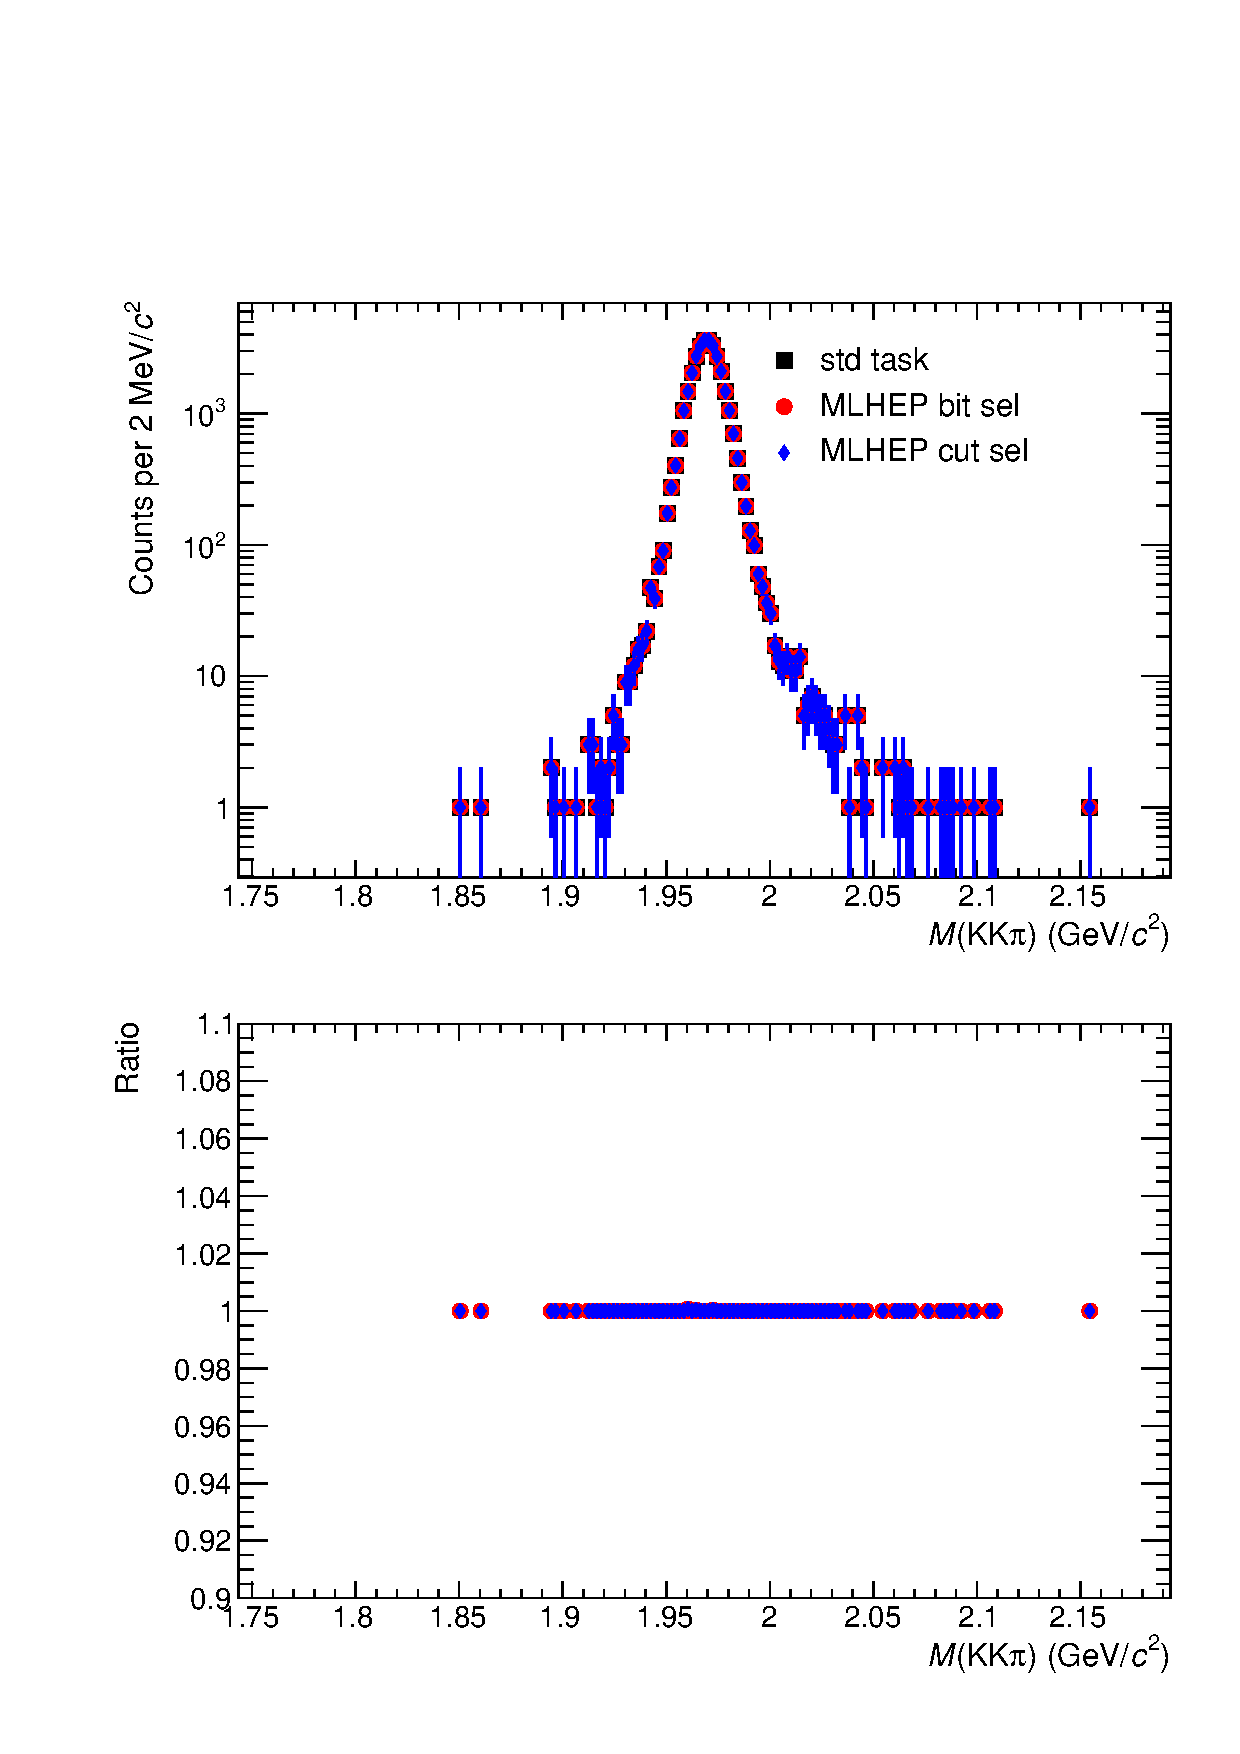
\includegraphics[width=0.5\textwidth]{figures/DsInvMassComparison.pdf}
\caption{Invariant-mass distribution of of signal (prompt and feed-down) $\Ds$ candidates with $2<\pt<24~\GeV/c$ obtained from the LHC18a4a2 MC production for pp collisions at $\sqrt{s}=5.02~\TeV$ with the AliAnalysisTaskDs task and the MachineLearningHEP package. The same selections used in~\cite{Acharya:2019mgn} were applied.}
\label{fig:InvMassDsComparisonMCpp} 
\end{center}
\end{figure}

- Lc in PbPb 2015 from TreeCreator compared to Lc published (raw signal per event)

\subsection{Efficiency}
\label{subsec:effValidation}

- Comparison efficiency from the package and RecoPID/GenLimAcc from correction framework

\begin{figure}[tb]
\begin{center}
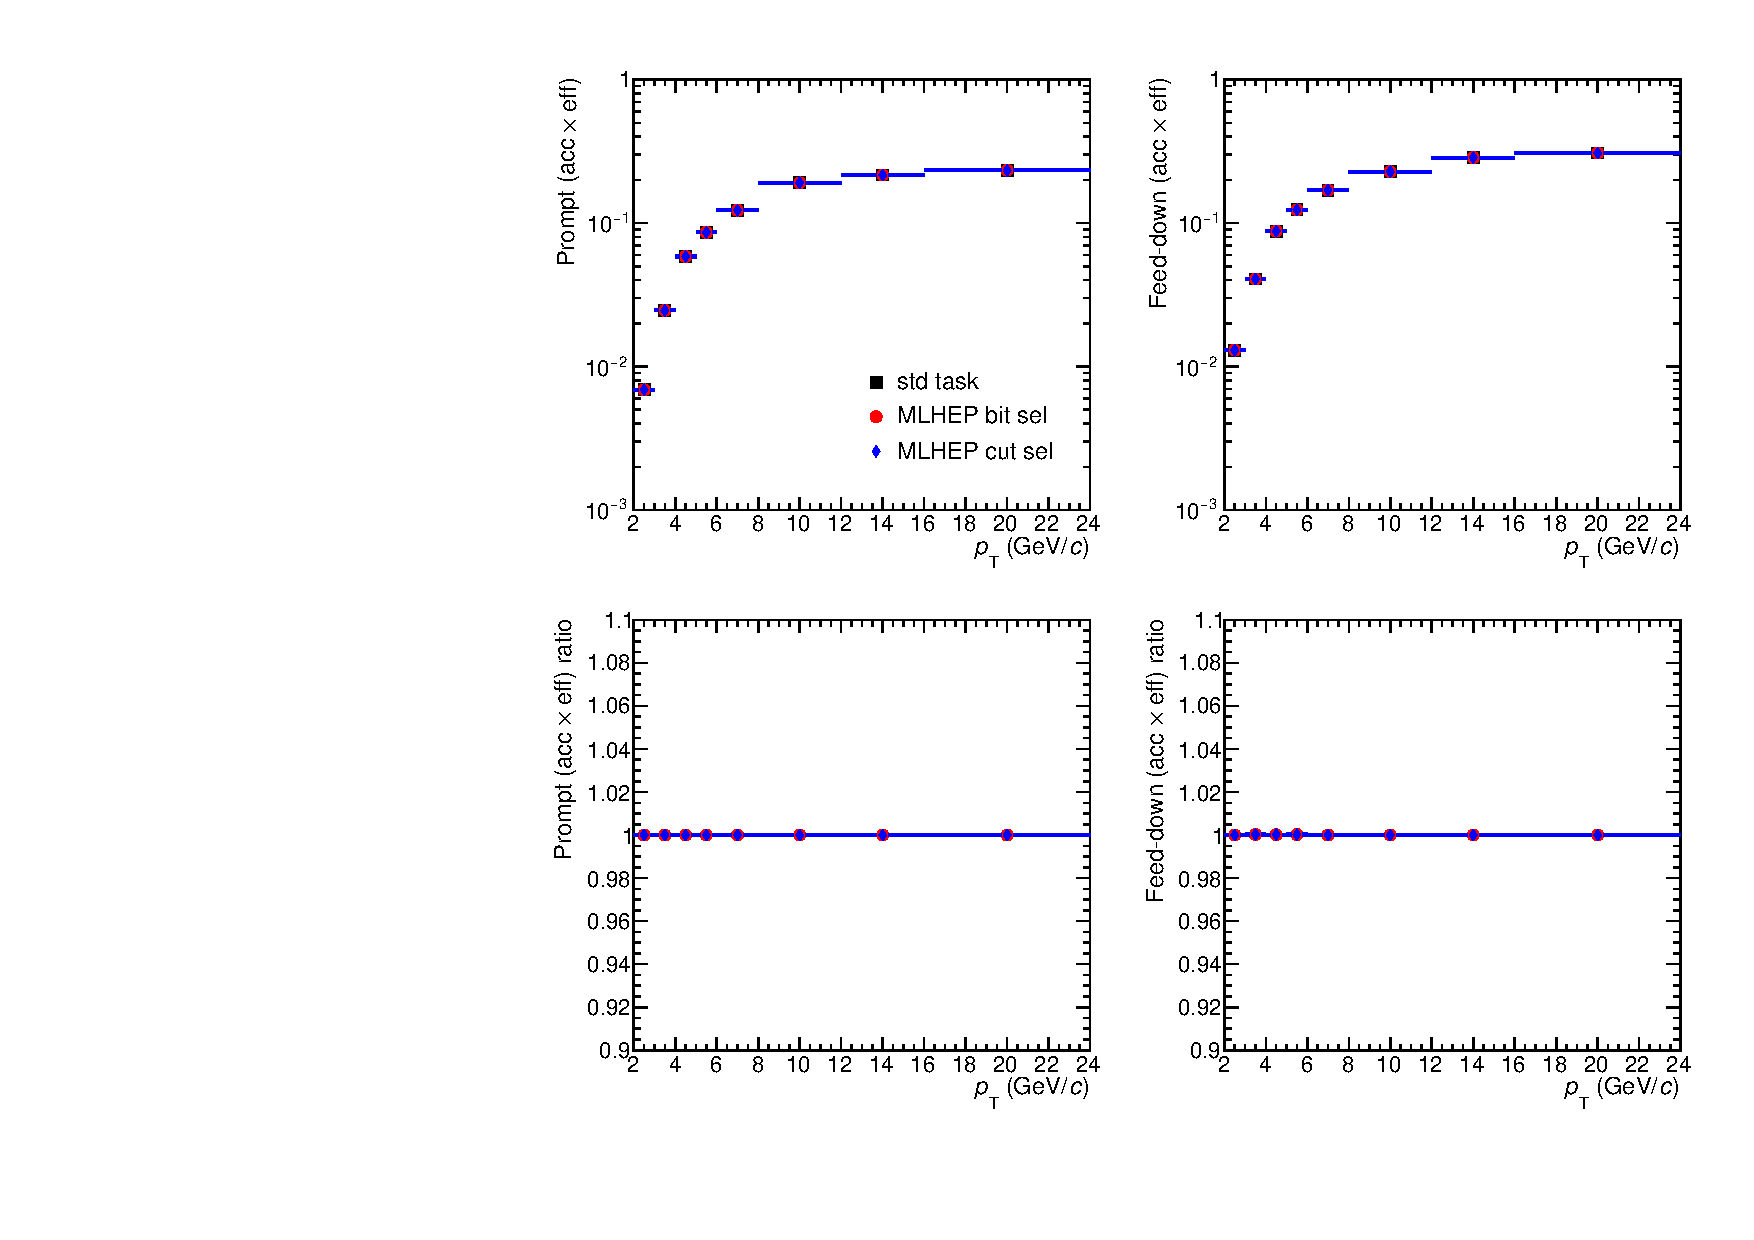
\includegraphics[width=0.9\textwidth]{figures/DsEfficiencyComparison.pdf}
\caption{Acceptance times efficiency factors of prompt (left) and feed-down (right) $\Ds$ with $2<\pt<24~\GeV/c$ obtained from the LHC18a4a2 MC production for pp collisions at $\sqrt{s}=5.02~\TeV$ with the AliAnalysisTaskDs task and the MachineLearningHEP package. The same selections used in~\cite{Acharya:2019mgn} were applied.}
\label{fig:EffDsComparisonMCpp} 
\end{center}
\end{figure}

\subsection{Normalisation}
\label{subsec:normValidation}

The number of events used to compute the integrated luminosity, which enters in the calculation of the cross section, calculated by the new framework is compared to the number obtained from AliNormalizationCounter (PWGHF/vertexingHF/AliNormalizationCounter.h). The number of events selected by AliRDHFCuts::IsEventSelected is corrected to take into account the events for which the primary vertex is not reconstructed and $|z_{vtx}|<10$~cm. 
 
 \begin{figure}[tb]
\begin{center}
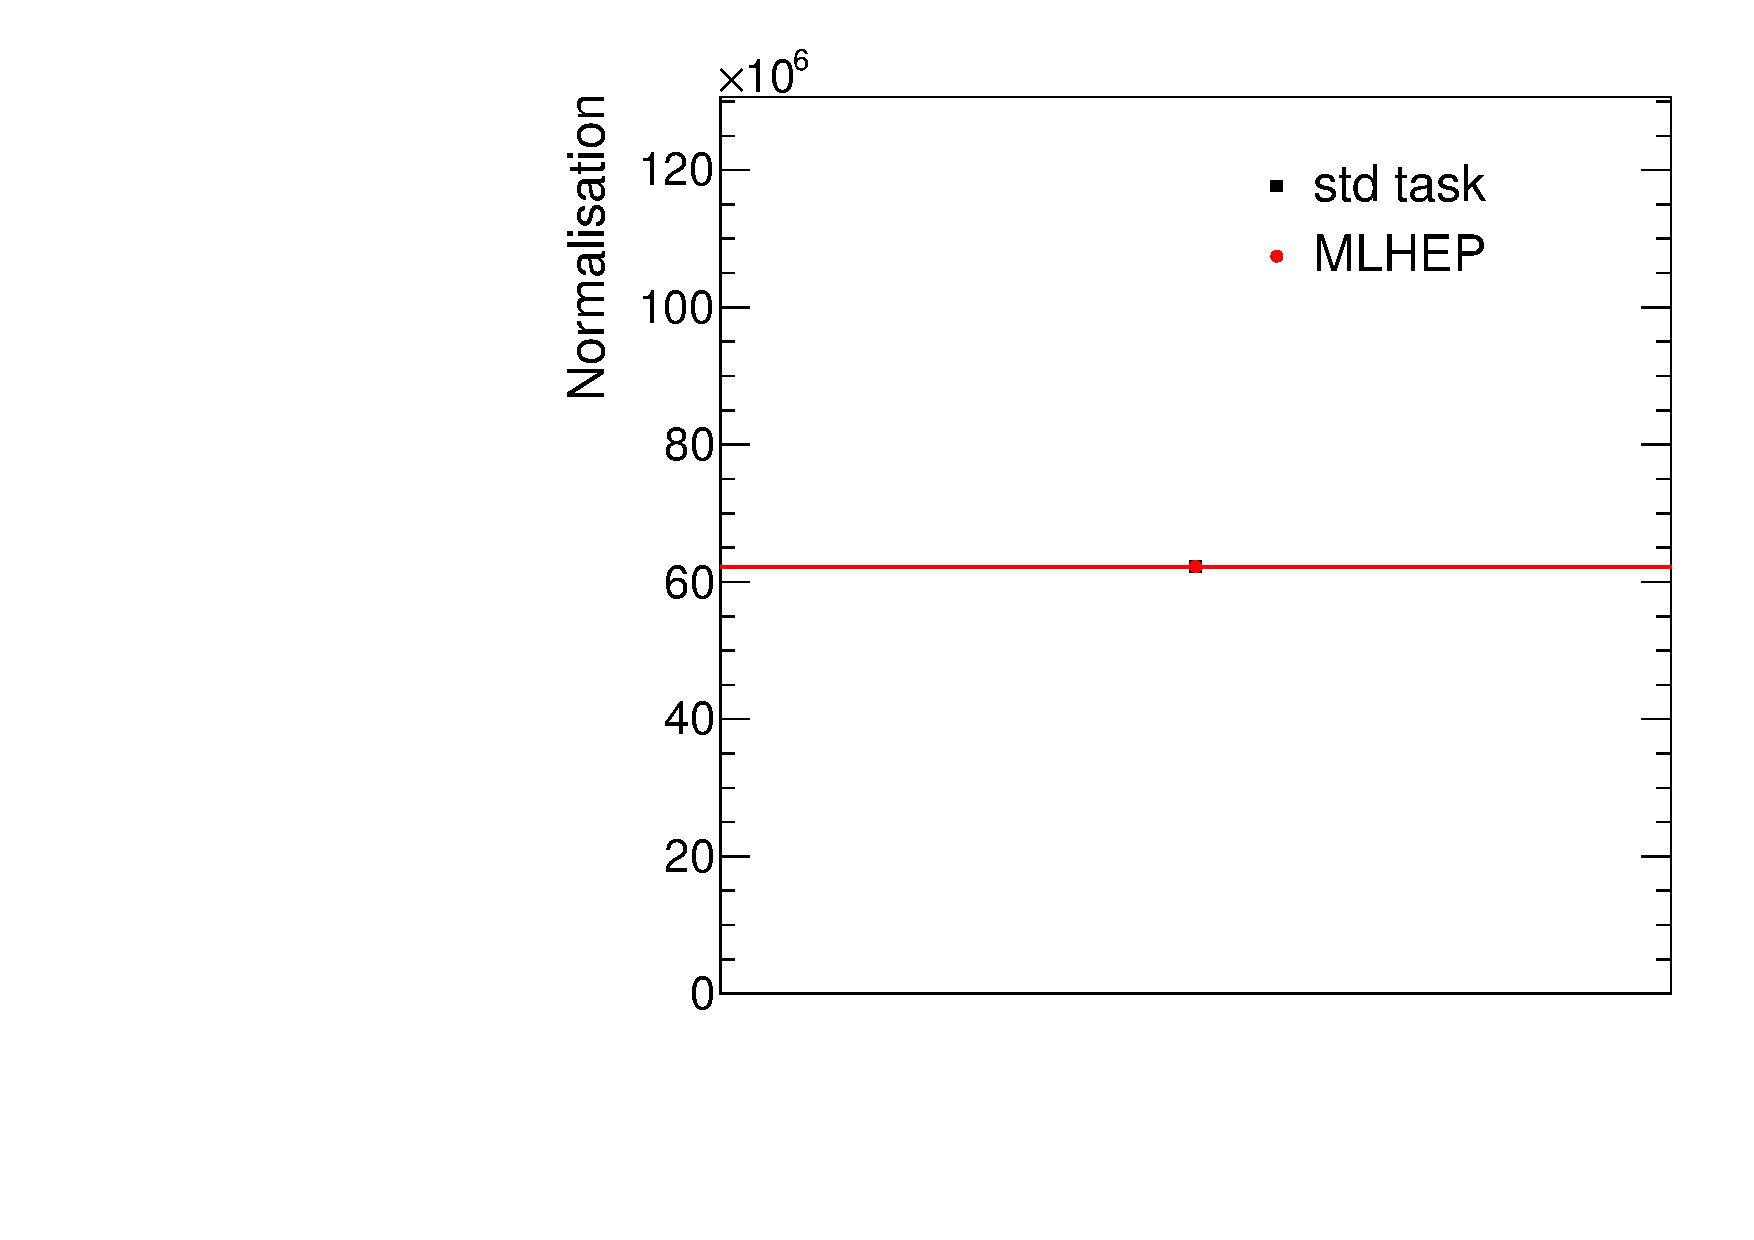
\includegraphics[width=0.5\textwidth]{figures/NormComparison.pdf}
\caption{Comparison of the normalisation factor obtained from the LHC18a4a2 MC production for pp collisions at $\sqrt{s}=5.02~\TeV$ with the AliNormalizationCounter and the MachineLearningHEP package.}
\label{fig:NormalisationComparisonMCpp} 
\end{center}
\end{figure}

- Ds in pp (running Tree Creator and std task in the same train)
- Lc in PbPb comparison of the events for normalisation/event selected from TTree and from task
